\section{NP-Hardness}

\subsection{A Game You Can't Win}
Given a box with $n$ binary switches and a light bulb.
Inside the box is a boolean circuit, s.t
\begin{itemize}
    \item \textsc{And}, \textsc{Or}, \textsc{Not} gates, as shown in \cref{fig:gates};
    \item $n$ input wires, one per switch;
    \item Gates connected to single output, i.e the light bulb.
\end{itemize}
\begin{figure}[H]
    \centering
    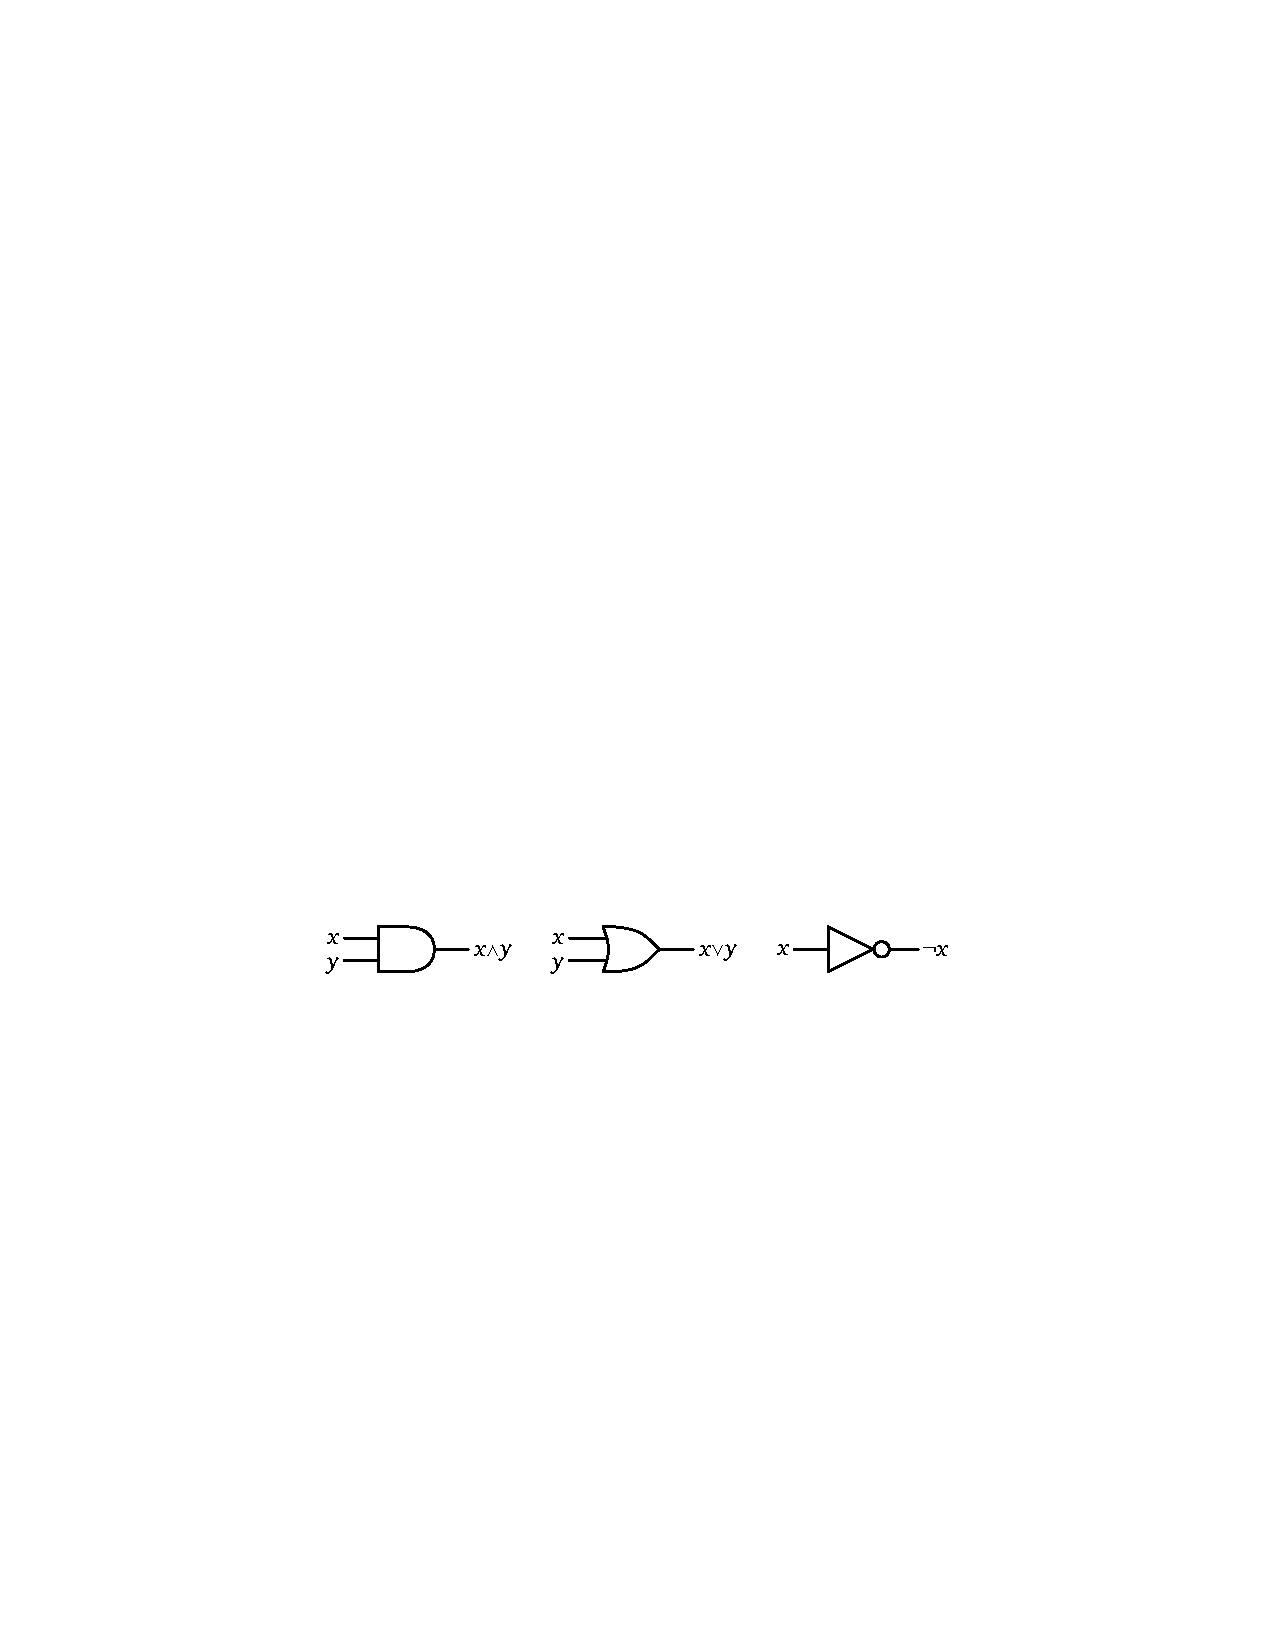
\includegraphics{fig/gates}
    \caption{An \textsc{And}, an \textsc{Or}, and a \textsc{Not} gate}
    \label{fig:gates}
\end{figure}
An example is shown in \cref{fig:lightbulb}
\begin{figure}[H]
    \centering
    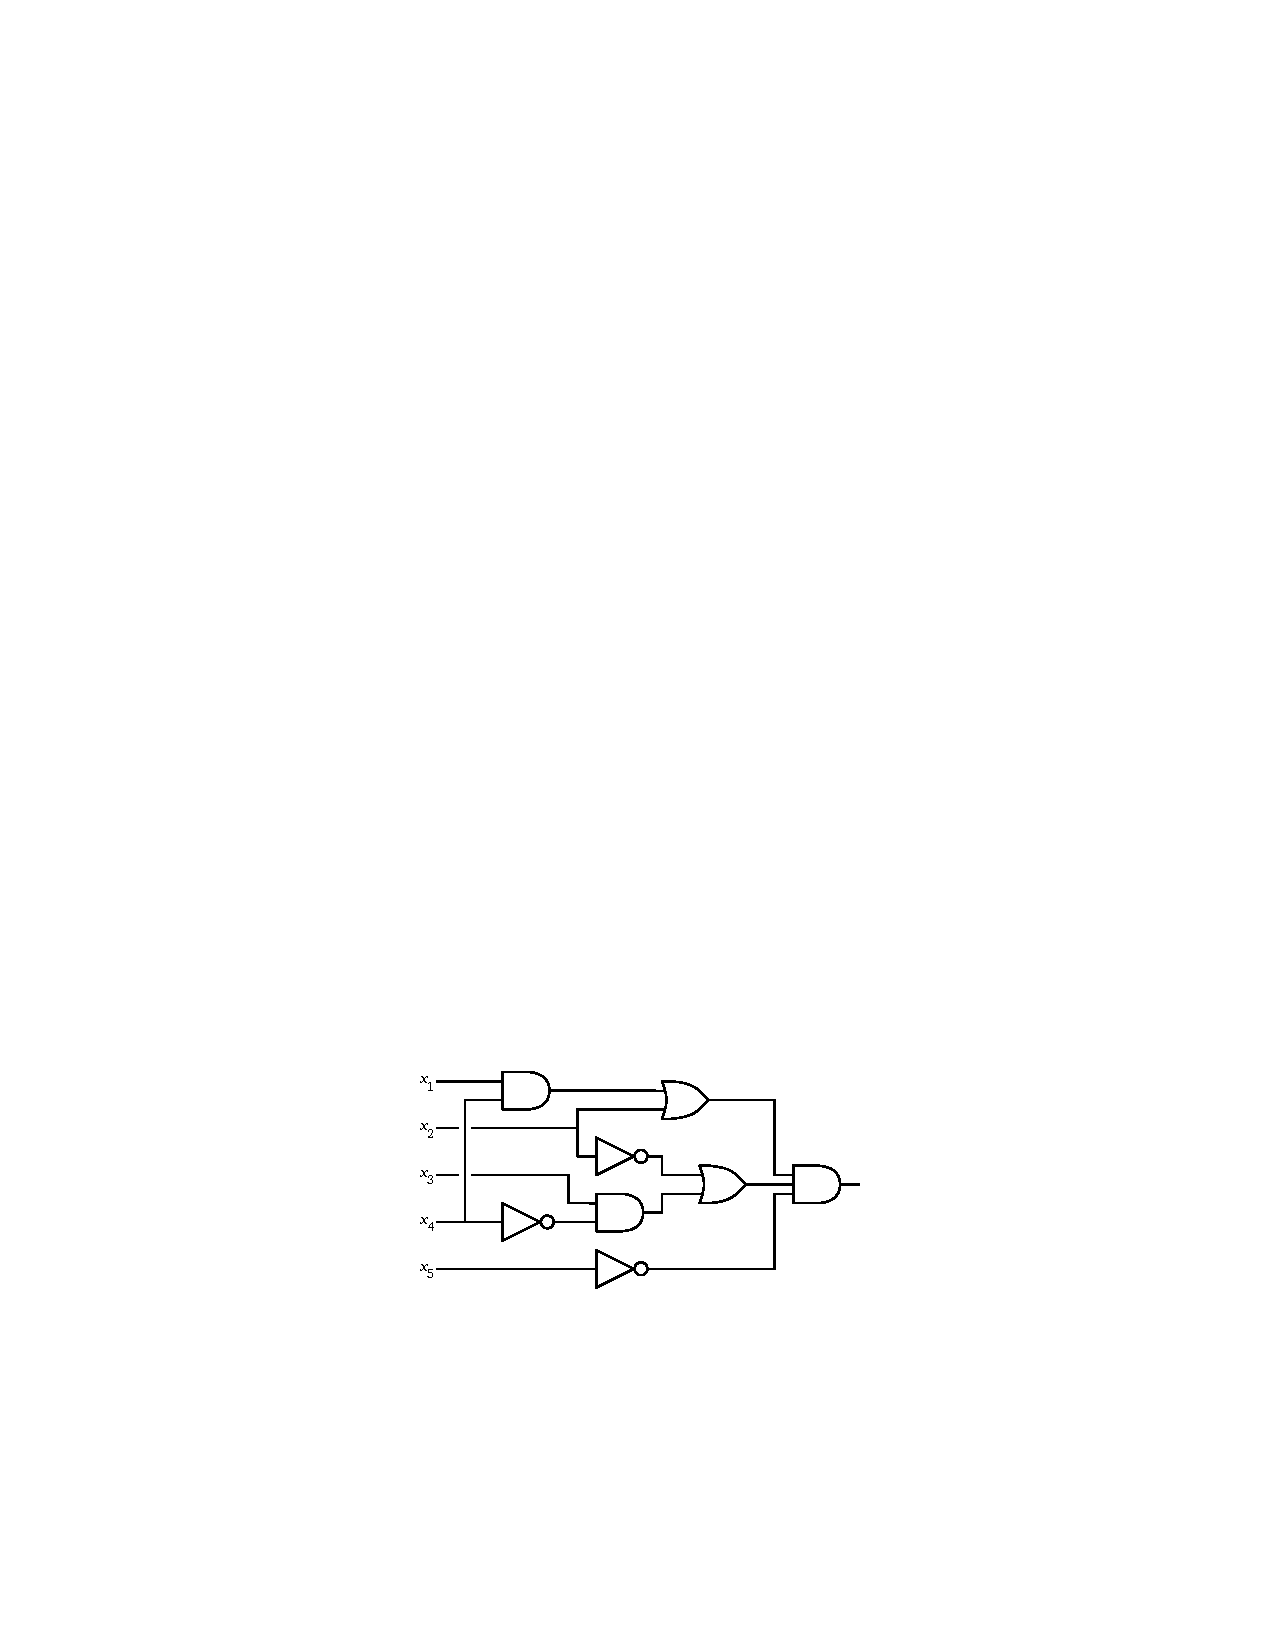
\includegraphics[scale=1.5]{fig/lightbulb}
    \caption{A boolean circuit}
    \label{fig:lightbulb}
\end{figure}
We want to know if there is a way to set switches s.t
light bulb turns on.
There are $2^n$ possible binary inputs. There is an \bigO{n} size circuit
which accepts a single strings and rejects all others.
Hence, if you cannot see inside, in worst case you must try all $2^n$ strings.

Suppose now you can see inside box. Can you do better than guessing all strings?
The answer is nobody knows for sure but many believe not.

The problem of determining if boolean circuit has satisfying assignment is all
\textsc{CircuitSAT}.

\subsection{P versus NP}
Minimum for an algorithm to be efficient is that it runs in polynomial time,
i.e \bigO{n^c} for constant $c$, $n$ is input size.
In this course, we focused on problems with polynomial solutions where $c$ is small.
\begin{itemize}
    \item Some problems known to require exponential time, i.e \bigO{c^n}, $c>1$.
    \item Some problems cannot even be solved (for example, Halting Problem).
    \item Some problems we don't know how hard.
\end{itemize}
NP-hard is a class most believe cannot be solved in polynomial time,
but no one knows for sure.

A decision problem is a problem whose output is a single boolean value,
i.e. \textsc{Yes/No}.
For example: LIS was an optimization problem. $\rightarrow$ ``Is there any increasing sequence of length $\geq k$?''
is a decision problem.
\begin{itemize}
    \item[P] Set of decision solvable in polynomial time, i.e ``efficiently solvable''.
    \item[NP] Decision problems s.t if answer in \textsc{Yes}, then there is a proof
        that can be checked in polynomial time. $\rightarrow$ can verify \textsc{Yes} if proof given to us.
    \item[Co-NP] Decision problems s.t if answer in \textsc{No}, then there is a proof
        that can be checked in polynomial time. $\rightarrow$ can verify \textsc{No} if proof given to us.
\end{itemize}
\textsc{CircuitSAT} is in NP, if satisfying string, then given string, it is easy to verify.

Why do most believe $P \neq NP$?
One intuition is that: solving problems is harder than verifying solutions.
\begin{itemize}
    \item[P] Problem in CLRS that you can solve quickly.
    \item[NP] Problem in CLRS that you can verify solution quickly.
\end{itemize}

\subsection{NP-Hard/NP-Complete}
A problem $\Pi$ is NP-hard if a polynomial time algorithm for $\Pi$ implies
polynomial time algorithm for all problems in NP.
\begin{quote}
    $\Pi$ is NP-hard $\leftrightarrow$ If $\Pi$ solution in polynomial time, then P = NP.
\end{quote}

Hence, most believe no NP-hard problem solvable in polynomial time.

$\Pi$ is NP-complete if $\Pi$ is NP-hard and $\Pi \in \text{NP}$.

Thousands of problems have been shown to be NPC.
How does one prove something NP-hard or NPC?

\begin{theorem}[Cook-Levin Theorem] \textsc{CircuitSAT} is NPC.\end{theorem}

All problems that are shown to be NPC, reduce from \textsc{CircuitSAT}.

\subsection{Reductions}
To prove any problem other than the \textsc{CircuitSAT} is NP-hard, use reduction.
Reducing problem A to problem B means solving A using solution for B.
To prove B is NP-hard, reduce \underline{from} known NP-hard problem A \underline{to} problem B.
Require reduction to be polynomial time in the A instance size.

Intuition: we are sure A is hard, Hence B must be hard, since otherwise it implies A can be
solved quickly.

Often write: $B \geq_p A$,
$\geq_p$ stands for B at least as hard as A ignoring polynomial factor.

A may still require more time to solve bu not more than polynomial factor.
